\documentclass[a4paper, 12pt, titlepage]{article}
%=======Unpackage Things===============
\usepackage{array}
\usepackage{color}
\usepackage{colortbl}
\usepackage{float}

\usepackage{graphicx}
\usepackage{amsmath}
\usepackage{amsthm}
\usepackage{listings}
%\usepackage{fullpage}
\usepackage{epsfig}
\usepackage{latexsym}
\usepackage{amssymb}
\usepackage{amstext}
\usepackage{enumerate}
\newcommand{\PreserveBackslash}[1]{\let\temp=\\#1\let\\=\temp}
\newcolumntype{C}[1]{>{\PreserveBackslash\centering}p{#1}}
\newcolumntype{R}[1]{>{\PreserveBackslash\raggedleft}p{#1}}
\newcolumntype{L}[1]{>{\PreserveBackslash\raggedright}p{#1}}


\begin{document}
\section{Linear and Polynomial Regression}
\begin{enumerate}[(a)]
        \item Load traning set and plot 
            \begin{figure}[H]
                \centering
                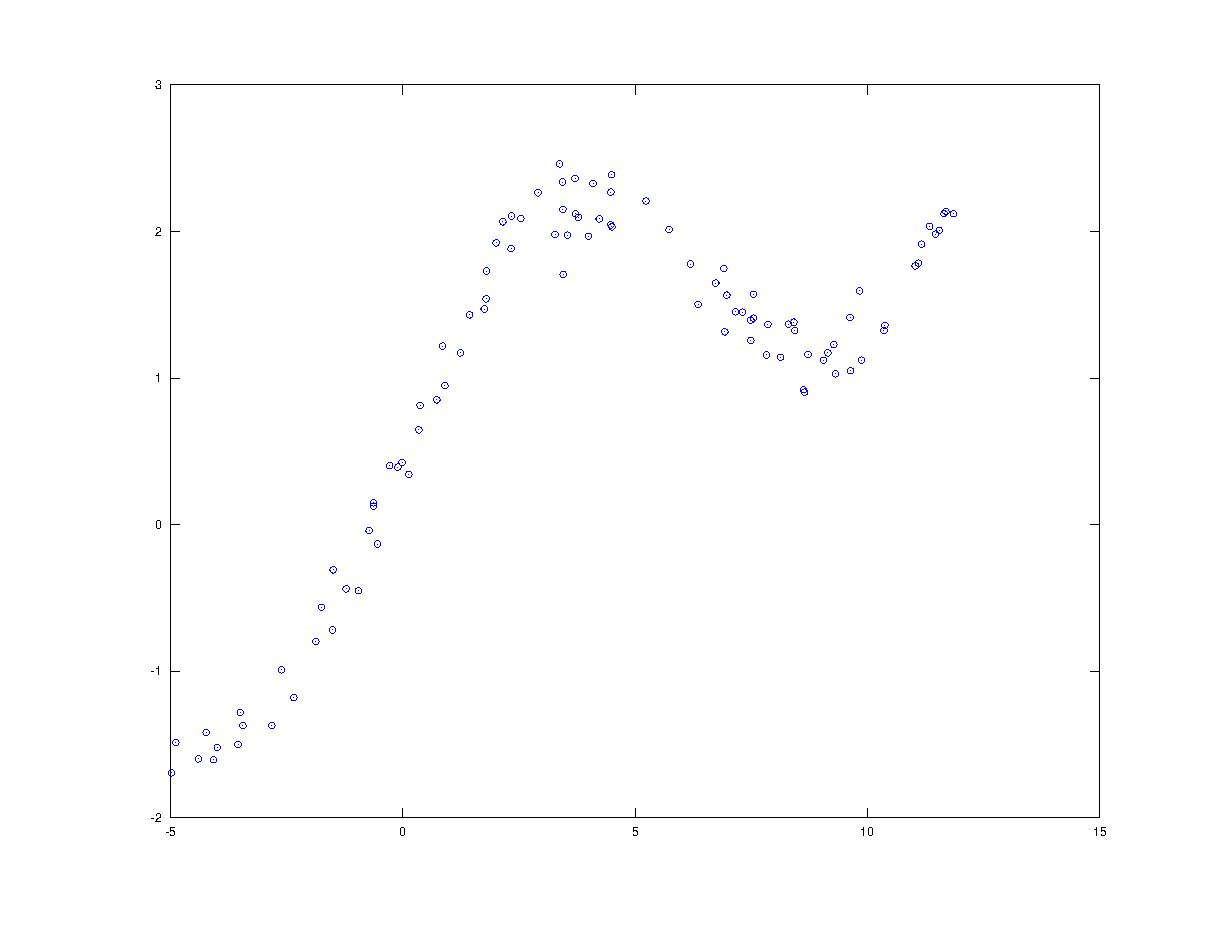
\includegraphics[width=8cm]{fig/a.eps}
                \caption{Plot Training Set}\label{a}
            \end{figure}
        
        \item Add a column of 1s and perform linear regression
            \begin{figure}[H]
                \centering
                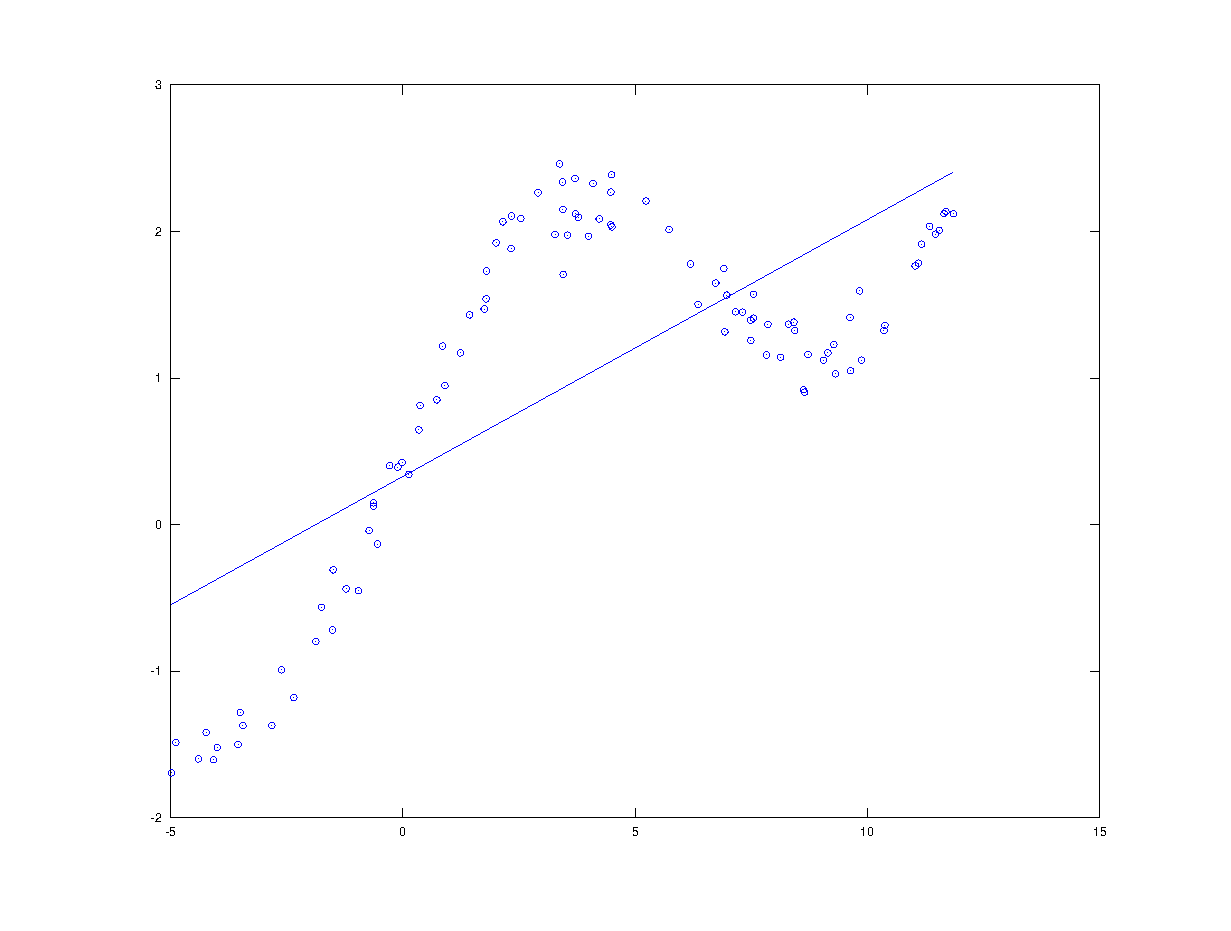
\includegraphics[width=8cm]{fig/linear.eps}
                \caption{Linear Regression}\label{b}
            \end{figure}

        \item The error function I used is \emph{sum-of-squares} function.
            $$J(w)=\frac{1}{2}\sum^m_{i=1}(h_w(x_i)-y_i)^2$$
            The function is implemented in J.m, which takes X, Y and W as parameters.

            The error of linear regression is 33.336445.
        \item The polynomial regression is implemented in PolyRegress.m
        \item Quadratic regression
            \begin{figure}[H]
                \centering
                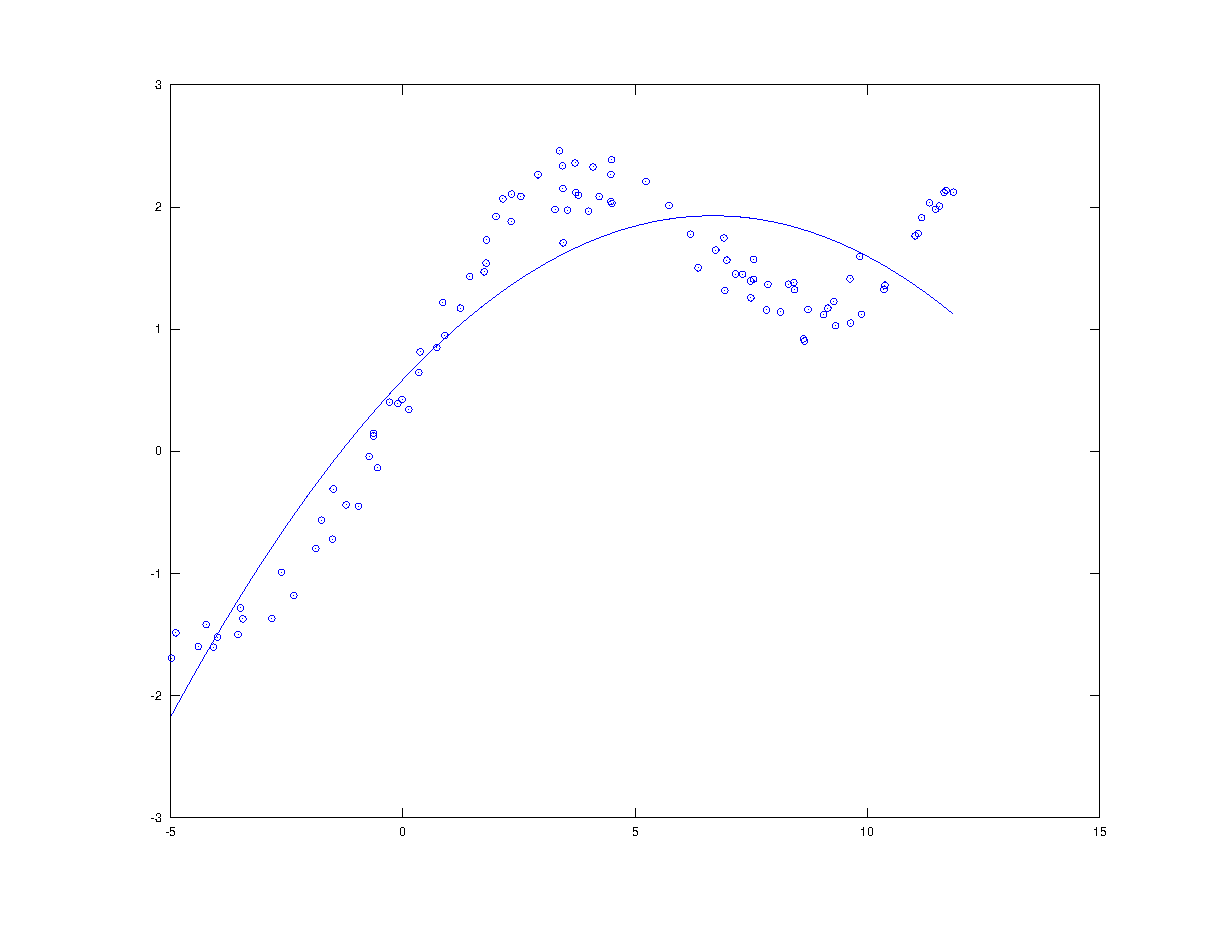
\includegraphics[width=8cm]{fig/quad.eps}
                \caption{Quadratic Regression}\label{e}
            \end{figure}

            error = 12.613

            Obviously, it is a better fit than linear regression.

        \item Cubic Regression %(f)
            \begin{figure}[H]
                \centering
                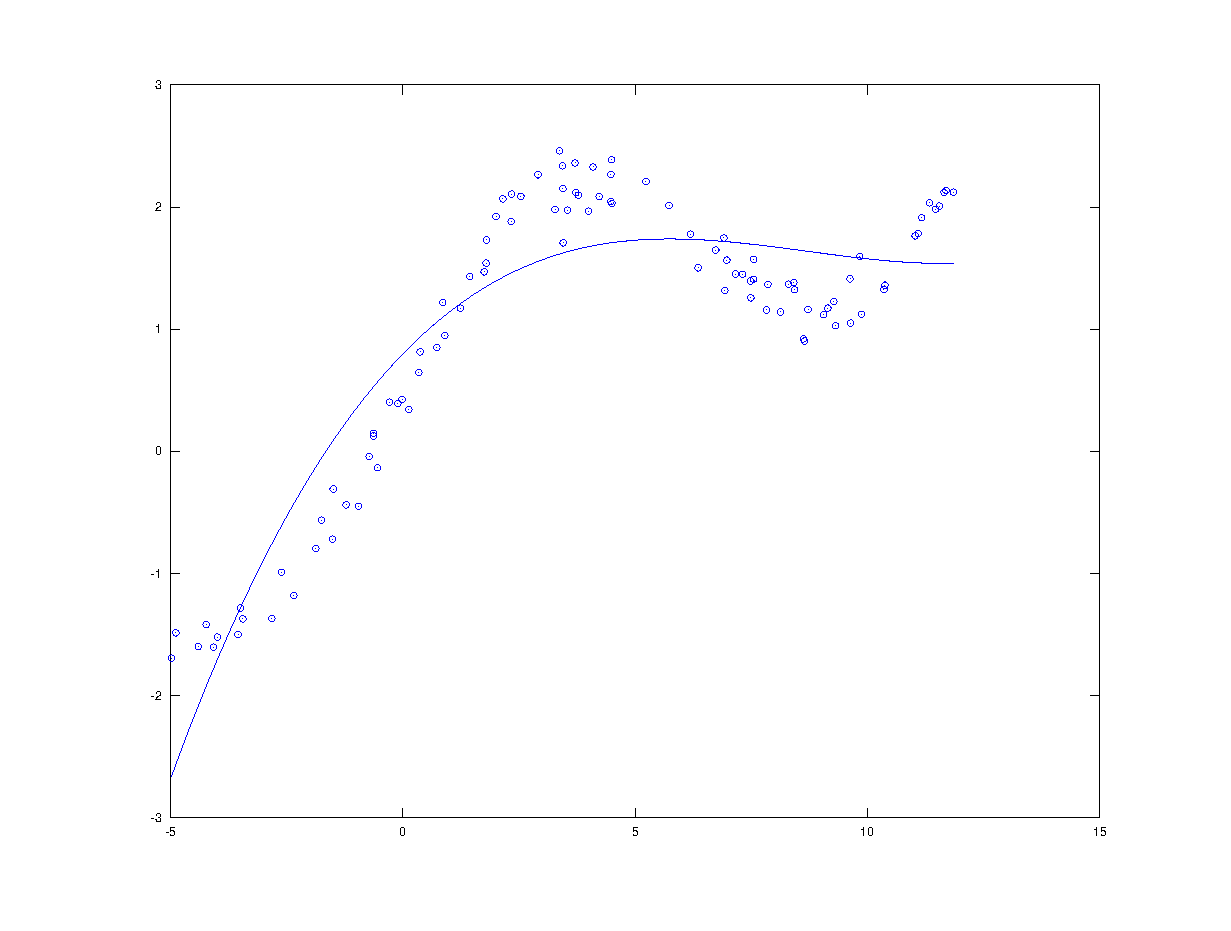
\includegraphics[width=8cm]{fig/cubic.eps}
                \caption{Cubic Regression}\label{f}
            \end{figure}

            Error = 10.878

            Comparing with the cubic regression, it is a better fit.

        \item %(g) 
            Using K-fold cross validation would be able to find the best fit in the data. The average error on traning data will keep decreasing and the average test error will reach a minimum and bounce back with the increase of order.

            However, if we only pick the fold in increasing order, the data we picked is not i.i.d.

        \item Table \ref{CrossValid} are the average training errors and average test errors from order 1 to order 7. From the table we can observe that the average test error reaches its minimum at the order 6, which means that the best order of polynomial is 6.
            \begin{table}[H]
                \centering
                \begin{tabular}{ccc}
                Order & Average Traing Error & Average Test Error \\
                    \hline
                1 & 26.55568 & 6.92412 \\
                2 & 10.03406 & 2.65285 \\
                3 & 8.58810  & 2.47171 \\
                4 & 1.14900  & 0.33340 \\
                5 & 1.13820  & 0.33771 \\
                6 & 0.85694  & 0.26229 \\
                7 & 0.85157  & 0.27419 \\
                8 & 14.88149  & 4.17042\\
                9 & 36.07754  & 9.39602 \\
                10 & 49.34058  & 12.76735 \\
                \end{tabular}
                \caption{5-Fold Cross Validation}
                \label{CrossValid}
            \end{table}

            Figure \ref{f} plots the data and the result of 6-order polynomial regression.

            \begin{figure}[H]
                \centering
                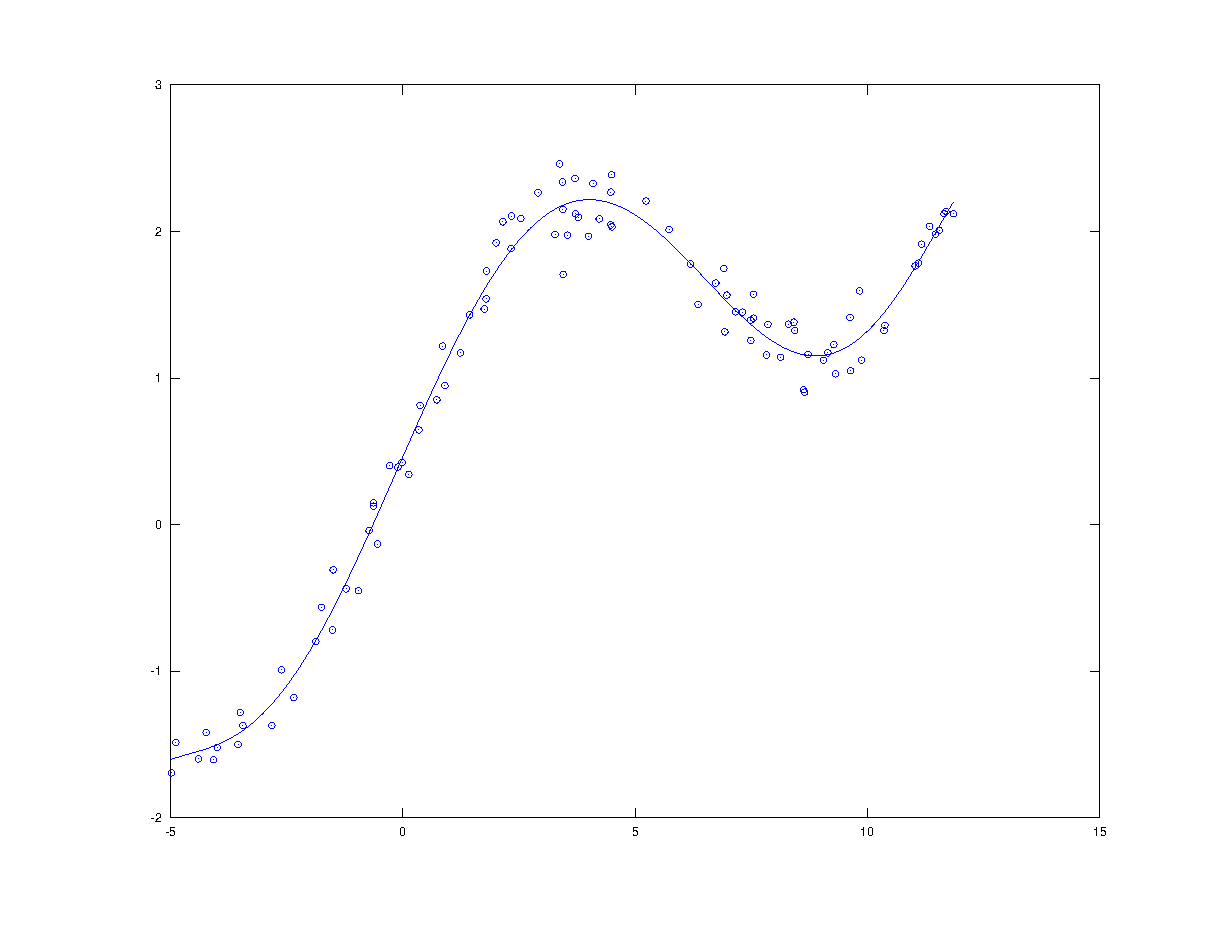
\includegraphics[width=8cm]{fig/6-order.eps}
                \caption{6-order Regression}\label{g}
            \end{figure}

            Error = 1.0936

        \item From table \ref{CrossValid}, we can observe that while the order is larger than 7, the error increased serviously. It is not what we expected and caused by numerical problem. In order to avoid such problem, normalization of input data is adopted. Table \ref{NCrossValid} is 5-fold cross validation with normalized data. Comparing with the previous table, the numerical problem does not happen anymore. And the approximator, i.e. the average errors, remain the same.
            \begin{table}[H]
                \centering
                \begin{tabular}{ccc}
                Order & Average Traing Error & Average Test Error \\
                    \hline
                1 & 26.55568 & 6.92412 \\
                2 & 10.03406 & 2.65285 \\
                3 & 8.58810  & 2.47171 \\
                4 & 1.14900  & 0.33340 \\
                5 & 1.13820  & 0.33771 \\
                6 & 0.85694  & 0.26229 \\
                7 & 0.85157  & 0.27419 \\
                8 & 0.84869  & 0.37166 \\
                9 & 0.83419  & 0.37078 \\
                10 & 0.82882  & 0.36763 \\
                \end{tabular}
                \caption{Normalized 5-Fold Cross Validation}
                \label{NCrossValid}
            \end{table}

            The best degree of polynomial regression, however, as same as the previous question, is still 6.

        \item Normalization have no effect on approximator

            


\section{Weighted Linear Regression}
\begin{enumerate}[(a)]
    \item In order to add weight matrix $U$ to the system, the matrix can be formed like this:
    \[ U = 
    \left| 
    {\begin{array}{ccccc}
    u_1 & 0 & 0 & \cdots & 0 \\
    0   & u_2 & 0 & \cdots & 0 \\
    0   & 0 & u_3 & \cdots & 0 \\
    0   & 0 & 0 & \ddots & 0 \\
    0   & 0 & 0 & \cdots & u_m
    \end{array}}
    \right|
\]
$Xw-y$~ can be represent in Matrix form:
\[Xw-y=
\left|
{\begin{array}{c}
    W^Tx_1-y_1\\
    W^Tx_2-y_2\\
    W^Tx_3-y_3\\
    W^Tx_4-y_4\\
    W^Tx_m-y_m
\end{array}}
\right|
\]
Thus, the cost function can be expanded like this:

$$J(w)=\sum_{i=1}^mu_i(w^Tx_i-y_i)^2 $$
$$J(w)=u_1(w^Tx_1-y_1)^2+u_2(w^Tx_2-y_2)^2+\cdots+u_m(w^Tx_m-y_m)^2$$
$$J(w)=(Xw-y)^TU(Xw-y)$$
    \item In order to calculate the gradient of J(w), we need to expand it:
        $$J(w)=w^TX^TUXw-w^TX^Tuy-y^TUXw+y^TUy$$
        Calculate the gradient:
        $$\nabla_wJ(w)=2X^TUXw-wX^TUy$$
        Set gradient to 0:
        $$\nabla_wJ(w)=2X^TUXw-wX^TUy=0$$
        $$w=(X^TUX)^{-1}X^TUy$$

\item

\end{enumerate}
\section{Error Criterion for Exponential Noise}

In order to find the best hypothesis $h$ on training data $D$, we need to find a hypothesis that maximum a psteriori:
$$h_{MAP}=\arg\max_{h\in{}H}P(h|D)$$
Using Bayes theorm
$$h_{MAP}=\arg\max_{h\in{}H}\frac{P(D|h)P(h)}{P(D)}$$
Since $D$ is independent of $h$
$$h_{MAP}=\arg\max_{h\in{}H}P(D|h)P(h)$$
If we assume all hypothesis are equally likely a priori, than we can further simplify and choose the maximum likelihood hypothesis:
$$h_{ML}=\arg\max_{h\in{}H}P(D|h)=\arg\max_{h\in{}H}L(h)$$

Adopt the assumption that:
$$y_i=h_w(x_i)+\lambda_i$$
where $\lambda_i$ is exponential distribution.
$$
    p_\lambda=\begin{cases}
        \lambda{}e^{-\lambda{}t}&t\geq0 \\
        0&otherwise
    \end{cases}
$$
The best hypothesis maximizes the likelihood of $y_i-h_w(x_i)=\lambda_i$:
%$$L(w)=\prod_{i=1}^m\frac{1}{\sqrt{2\pi\sigma^2}}e^{-\frac{1}{2}(\frac{y_i-h_w(x_i)}{\sigma})^2}$$
$$L(w)=\prod_{i=1}^m\lambda\cdot{}e^{-\lambda(y_i-h_w(x_i))}$$
Apply the $\log$ trick
$$\ln{}L(w)=\sum^m_{i=1}(\ln\lambda-\lambda(y_i-h_w(x_i))\\
=\sum^m_{i=1}\ln\lambda-\sum^m_{i=1}\lambda(y_i-h_w(x_i))$$
We want to maximize the likelihood, thus we need to minimize $\sum^m_{i=1}\lambda(y_i-h_w(x_i))$. So, the error criterion we choose is:
$$w^*=\arg\min_w\sum^m_{i=1}\lambda(y_i-h_w(x_i))$$


\end{enumerate}
\end{document}
